\documentclass[UTF8]{ctexart}
%\title{HDFS海量小文件存取优化}
\newcommand{\horrule}[1]{\rule{\linewidth}{#1}} % Create horizontal rule command with 1 argument of height
\title{
  \normalfont \normalsize 
  \textsc{\\~\\~\\~\\~\\~\\University of Science and Technology of China} \\ [25pt] % Your university, school and/or department name(s)
  \horrule{0.5pt} \\[0.4cm] % Thin top horizontal rule
  \huge 基于LSTM的DFS小文件存取优化 \\ % The assignment title
  \horrule{2pt} \\[0.5cm] % Thick bottom horizontal rule
}
\newcommand{\n}{\\\indent}
%\author{\Large{阮震元~~~~解宇飞~~~~杨智~~~~刘旭彤}\footnote{阮震元~:~PB13011009,联系方式rzyrzyrzy2014@gmail.com,科技实验楼1406系统设计室}
%\setcounter{footnote}{-1}
%\footnote{解宇飞~:~PB13011001~~~~杨智~:~PB13011079~~~~刘旭彤~:~PB13011072}
%\footnote{董恒   李楠    连家诚}

%\author{董恒}
\date{\today}
\usepackage{graphicx}
%\usepackage{listings}
%\usepackage{minted}


\begin{document}
\maketitle
\clearpage
\tableofcontents
\clearpage
\section{小组成员}
简单介绍一下小组的成员

\paragraph{董恒}
C、C++、python编程经验,未做过大型项目。对神经网络有一些了解。

\paragraph{李楠}
C、C++ 编程经验。

\paragraph{连家诚}
C、C++ 编程经验,学过单片机开发。

\paragraph{小结}
总的来说,我们3个人均不是大佬级别的人物,没有太多的背景支持,所以关于这个课题的东西基本上都需要从零开始。






\section{项目背景}
本节介绍这个课题的相关背景,包括分布式文件系统概述,HDFS的介绍,其他分布式文件系统介绍。

\subsection{分布式文件系统}
简介什么是分布式文件系统以及它的特点和简要历史。

\subsubsection{简介}
分布式文件系统(Distributed File Systen)是指文件系统管理的物理存储资源不一定直接连接在本地节点上,而是通过计算机网络与节点相连。分布式文件系统的设计基于客户机/服务器模式。一个典型的网络可能包括多个供多用户访问的服务器。另外,对等特性允许一些系统扮演客户机和服务器的双重角色。

\paragraph{DFS与DAS的区别}Distributed file system和Distributed data store的区别是,前者允许使用同样的interfaces存取文件,就像操作本地文件,比如说:mounting/unmounting、列出目录、以byte读/写、 system's native permission model. 而Distributed data stores,需要使用一个不同的API或者库。

一个分布式文件系统也可以通过软件实现IBM的 Distributed Data Management Architecture (DDM) 来创建,这样的话,在一个计算机上运行的程序通过使用本地接口来创建、管理和存取在另一个计算机上的文件。所有这样的客户机需要使用被DDM定义的等价的信息。通过使用同样由DDM定义的协议,这些信息被传递到特定的远程计算机上,在远程计算机上,一个DDM程序解释这些信息,然乎使用文件系统接口来定位以及操作特定文件。

\subsubsection{设计目标}
分布式文件系统在很多方面都希望实现"transparency". 这是说,他们希望这些对客户机程序是不可见的,让客户机可以把DFS看成本地系统。在这种情况下,分布式文件系统处理定位文件、传递数据,以及可能提供其他的特性,列表如下:
\paragraph{Access transparency}
客户机并不会意识到文件是分布式的,它们能够像存取本地文件一样存取分布式文件。
\paragraph{Location transparency}
有一个一致的名字空间存在,包含了本地文件和远程文件。一个文件的名字不会提供具体的存储位置。
\paragraph{Concurrency transparency}
所有的客户机看到同样的文件系统状态。这就是说,如果一个进程修改了一个文件,任何其他的进程,不论它在相同的文件系统上还是远程系统上,都会看到看到修改。
\paragraph{Failure transparency}
如果一个服务器故障,客户机和客户机程序应该正确运行。
\paragraph{Heterogeneity}
文件服务应该可以提供给不同的硬件和操作系统。
\paragraph{Scalability}
文件系统应该能够在小规模环境(一个或几个机器)和大规模环境(成百上千的机器)中正常运行。
\paragraph{Replication transparency}
为了提供Scalability,文件系统需要在不同的服务器里复制文件,并且客户机不会意识到这一点。
\paragraph{Migration transparency}
文件应该可以自由移动。

\subsubsection{小历史}
1960s, Incompatible Timesharing System 为了实现不同机器间文件系统存取的透明性,使用了虚拟设备。
1970s, 更多的文件服务器被开发。
1976, Digital Equipment Corporation创建了 File Access Listener (FAL),作为 Data Access Protocol的一个实现,这个协议是DECnet Phase II的一部分,后来成为第一个被广泛使用在网络文件系统的协议。
1985,Sun Microsystems 开发了一个称为 "Network File System" (NFS)的文件系统,这个文件系统后来成为第一个被广泛使用的基于网络协议的网络文件系统。
其他著名的网络文件系统包括:Andrew File System (AFS), Apple Filing Protocol (AFP), NetWare Core Protocol (NCP), and Server Message Block (SMB),最后一个被称为Common Internet File System (CIFS).

1986,IBM宣称客户机和服务器支持Distributed Data Management Architecture (DDM)对于System/36, System/38, 以及跑CICS的IBM mainframe计算机. 后来也支持IBM Personal Computer, AS/400, 使用 MVS和VSE操作系统的IBM mainframe计算机以及FlexOS. DDM也成为 Distributed Relational Database Architecture(DRDA)的基础。

现在有许多的p2p网络协议,去支持开源分布式文件系统以及闭源集群式文件系统,比如 9P, AFS, Coda, CIFS/SMB, DCE/DFS, Lustre, Google File System, Mnet, Chord Project.



\subsection{常见DFS介绍}
以下简单介绍常见的DFS,其中HDFS留到下一节专门介绍。为了更加全面了解到现有分布式文件系统的特性,下面调研了维基百科上相关联的一些DFS. 为了便于后续的研究,这里只说明我们关注的方面,比如特性、使用、实现。

\subsubsection{GlusterFS}
\paragraph{去中心化的分布式元数据架构}
采用DHT的方式将每个file按照filename映射到节点上,通过Davies Meyer hash函数对filename取hash值如果file被rename,那么按照新的name计算hash后的新节点上会新建一个pointer,指向原来文件元数据所在节点。
\paragraph{模块化、协议栈式的文件系统}
目前支持三种基本的功能和属性:
                  Replicator         (副本,相当于raid1)
                  Stripe               (条带,相当于raid0)
                  Distributed     (分布式,相当于DHT)
以上任意两个模块可以组合在一起。当时系统一旦选择其中一个属性,后面不能再修改。
目前主要的用法是Distributed+Replicator。选择了Distributed+Replicator后,某个文件就会在Gluster集群的两个节点上各有一份镜像。
其他:
         存储节点上支持多种文件系统ext3、ext4、xfs、zfs.
         存储节点的硬件可以是JBOD,也可以是FC san.
         NAS集群功能通过CTDB实现.
         通过一个用户态的轻量级的nfsserver提供NFS接口.
         CIFS通过linux自带的Samba实现.
全兼容Hadoop,可以替代HDFS.
Client端提供最新的KVM的补丁,可以为KVM的虚拟机提供存储能力。
\paragraph{商业应用}
最初GlusterFS由Gluster INC提供商业服务。被intel收购后将全部源码开源。也有第三方的存储厂家提供基于GlusterFS的解决方案。

\subsubsection{Ceph}
Ceph主要架构来自于加州大学SantaCruz. 分校Sage Weil的博士论文。07年毕业后全职投入ceph的开发。12年才有stable版本发布。目前开发者社区是由Inktank公司主导并提供商业支持。
\paragraph{特点1}
采用集中式元数据管理,整体架构包括client(在kernel实现),MDS和OSD。文件目录树由MDS维护。文件被切分为大小相同的object,每个object被hash到不同的OSD(数据节点)上,OSD负责维护具体的文件数据。
\paragraph{特点2}
支持元数据服务器集群,将目录树动态划分为若干子树,每个子树都有两个副本在两个MDS上提供服务,一个MDS同时支持多个不同的子树:
\paragraph{特点3}
统一存储架构,支持多种接口。去掉MDS并增加若干Http proxy server后,就是P2P的对象存储,支持S3接口。去掉MDS并增加iSICSI Target Server还可以对外提供block接口。
\paragraph{特点4}
Ceph中的一致性通过primary副本来保护。每个对象有一个主副本,客户端只跟主副本打交道,主副本所在的OSD负责把数据写到其他副本。
\paragraph{特点5}
虚拟化环境的集成,支持多种元计算框架例如OpenStack、CloudStack、OpenNebula,Ceph已经可以集成到openstack作为cinder(弹性块存储,类似amazon的EBS)的一种实现。
\paragraph{商业应用}
目前ceph被视为一种实验性的文件系统,目前并无大型商业应用。根据Inktank公司公布的调查结果,目前在一些中小型的企业和组织中有商业应用,生产环境尚未有超过1P的案例。目前有些openstack厂家也在验证使用ceph为云计算环境提供虚拟化存储的可行性。

\subsubsection{Lustre}
Lustre是linux+cluster的缩写。Lustre是一个并行的分布式文件系统,主要应用领域是HPC(high performance compute)。目前Top100的超级计算机中,超过60的都是在使用lustre。
\paragraph{特点1}
传统的体系结构:MDS(元数据服务器) OSS(数据服务器)Client。MDS、OSS分别将元数据信息、数据信息持久化存储到本地文件系统中,本地文件系统采用的是ext4。每个文件会被切分成多个大小相等的object,多个object条带化到多个OSS上。MDS负责存储和管理file跟object映射关系。
\paragraph{特点2}
支持上万个客户端的并发读写。HPC领域的重要应用场景是多个客户端并发读写同一个文件。Lustre通过Distributed Lock Manager解决多客户端并发读写的问题。Lock包括两种,一个种是fileinode的锁,一种是file data的锁。Inode锁由mds统一管理,file data锁则由OSS管理,file data锁支持字节范围的锁。
\paragraph{商业支持发展}
最初组织Lustre开发的公司先被sun收购。Sun被oracle收购后大部分开发人员离开并组织了新公司,目前新公司已经被intel收购。由于lustre本身开源,传统SAN硬件厂家例如HDS、Dell、netapp也将lustre捆绑自己的硬件提供解决方案,并提供lustre技术支持。每年都会召一次全球Lustre用户大会LUG(lustre user group)。

\subsubsection{MooseFS}
MooseFS本质上是GoogleFS或HDFS的c实现。
       集中式元数据管理,元数据服务器主备。

MooseFS组成说明

\begin{tabular}{p{3cm}p{8cm}}
\hline
角色 & 角色作用 \\
\hline
managing server(master) & 负责各个数据存储服务器的管理,文件读写调度,文件空间回收以及恢复.多节点拷贝\\
\hline
Metalogger server(Metalogger)& 负责备份master 服务器的变化日志文件,文件类型为changelog\_ml.*.mfs,以便于在master server 出问题的时候接替其进行工作\\
\hline
data servers(chunkservers) & 负责连接管理服务器,听从管理服务器调度,提供存储空间,并为客户提供数据传输.\\
\hline
client computers & 通过fuse 内核接口挂接远程管理服务器上所管理的数据存储服务器,.看起来共享的文件系统和本地unix 文件系统使用一样的效果\\
\hline
\end{tabular}

\paragraph{Moosefs的功能特点}
支持snapshot.
         实现了文件回收站。
         支持动态扩容。
         小文件读写优化。
         Client支持多种操作系统包括:Linux FreeBSD OpenSolaris和MacOS
\paragraph{商业应用}
中小型企业,学校、web网站。
存放普通文件、img、weblog等分结构化数据。
Web server备份 。
Kvm xen虚拟机镜像文件。

\subsubsection{TFS}
TFS是淘宝开源出来的专门存储图片的分布式文件系统。
TFS的总体架构也是仿照HDFS,区别如下:

\begin{itemize}
\item HDFS中一个file由多个chunk组成。TFS反过来,一个64Mchunk会存放多个file。相当于小文件聚合。
\item TFS的filename包含了很多元数据信息力例如文件的chunkid和fileid,这样显著减轻了MDS的压力。
\item 文件在chunk中的偏移量mds不需要关心,具体维护是datanode来做的,减少了mds维护的元数据信息。
\item 为了防止磁盘碎片,datanode利用ext4的一些特性,例如fallocate,首先利用fallocate为每个chunk文件分配好空间。
\item Mds在为每个新文件分配chunk时,采用的是一致性hash的方法定位新chunk的位置。这样有利于集群的线性扩容。
\end{itemize}

\subsubsection{Fast DFS}
Fast DFS是一种纯轻量级的分布式文件系统,主要有国内开发者贡献。主要特点是结构简单,维护成本低,一般用于小型网站。架构特点:

\begin{itemize}
\item 不维护目录树,client每次新建文件的时候由负载均衡器Tracker Server生成一个file id和path给client
\item 没有file和chunk概念,Tracker server只是负责轮选storage server给client使用。
\item Storage server分成不同的group,每个group之间是简单的镜像关系。
\item 读写文件时tracker负责不同组以及组内的负载均衡。
\item Strage server就是把文件写入到本地的文件系统中。
\end{itemize}


\subsection{HDFS}
以下内容主要来自\cite{Dhruba},作为专门讲解HDFS结构的文献,这篇文章讲得比较详细,整理如下。
\subsubsection{Intro}
HDFS 被设计为可以运行在商用硬件上,与现存的分布式文件系统有很多的相似之处。但是区别也很明显,比如高容错性,高吞吐率。这一点也让HDFS非常适合大数据存取。

HDFS基本实现了以下的几个特点:
\paragraph{硬件故障}
HDFS由很多机器构成,这种情况下,硬件故障将成为一种常态,所以系统必须能够检测到故障并且能够快速自动恢复。

\paragraph{流数据存取}
在HDFS上运行的应用需要流存取数据集,并且系统更多地被设计成为了批处理而不是交互式使用,所以更多地需要数据的大吞吐率。

\paragraph{大数据集}
在HDFS上运行的应用需要大数据集,每一个文件大概是GB到TB大小,因此系统需要提供大的数据带宽。

\paragraph{简单连接模型}
基本模型是: write-once-read-many存取模型。一个文件一旦被创建、写入然后关闭之后就不必被改变。这样的假设简单化了模型,并且使高吞吐率成为可能。

\paragraph{移动计算而不是移动数据}
让计算更加接近数据会更加高效,特别是当数据量很大时。这种方式减少了网络拥挤并且提高了系统总的吞吐率。一种假设是,移动计算到接近数据的位置比移动数据到应用运行的位置更加合适。因此,HDFS 提供了一种让应用移动它们自己到数据存储位置的接口。

\paragraph{可移植性}
HDFS设计成很容易从一个平台移动到另一个平台。

\subsubsection{NameNode和DataNode}
HDFS有一个master/slave结构,一个HDFS集群由一个NameNode和几个DataNode组成,其中NameNode是一个master服务器,管理文件系统命名空间以及管理客户机的存取,DataNode管理储存。在内部,一个文件被分割成一个或者几个块,这些块被存储在一些DataNode中。NameNode处理文件系统命名空间的操作,比如说,打开、关闭、重命名文件或者目录,并且NameNode也决定了块到DataNodes的映射关系。DataNode则处理客户机的读写请求,以及块的创建、删除和复制。下面的图\ref{fig:HDFS_Arch}形象表示了这种结构。

\begin{figure}[h]
\centering
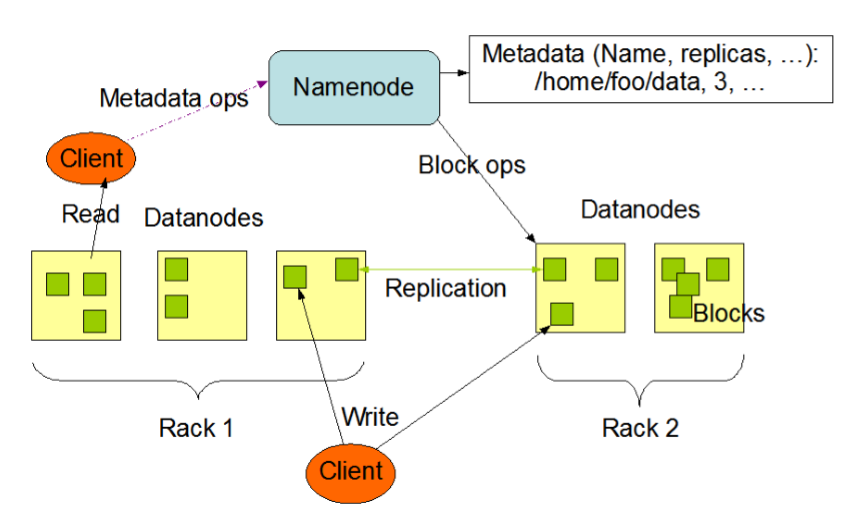
\includegraphics{HDFS_Arch.PNG}
\caption{HDFS Architecture}
\label{fig:HDFS_Arch}
\end{figure}

NameNode和DataNode都是一些能在商用机器上运行的软件。可用Linux,由于HDFS使用Java实现,因此任何支持Jave的机器可以运行NameNode和DataNode.

\subsubsection{文件系统命名空间}
HDFS支持一个传统的文件组织体系,一个用户或者一个应用额可以创建目录然后储存文件。文件系统命名空间和现有的文件系统非常相似,可以创建、移除文件,移动文件到另一个目录,或者重命名一个文件。但是HDFS并未实现用户限额和存取许可,以及硬链接、软链接也不支持。但是HDFS的结构并不排除实现这个功能。

NameNode维持文件系统的命名空间,任何对文件系统命名空间的修改都会被NameNode记录,

\subsubsection{数据复制}
HDFS被设计成能够可信地在一个大集群内存储大容量数据,它把一个文件存储在连续的几个块中,除了最后一个块外,其他的块都由同样的大小。为了实现容错性,块都会被复制存储。每个块的大小和复制数都可以被设置,在创建的时刻或者在之后。HDFS文件每次只能有一个写入。NameNode处理所有的关于块复制的决定,它会周期地从每个DataNode收到一个心跳和一个块报告,心跳代表NameNode正常运行,块报告包含了在一个DataNode里面所有的块的列表。

\subsubsection{文件系统元数据的存储}
HDFS命名空间被存储在NameNode,NameNode使用信息日志(EditLog)来记录每次元数据的改变。比如说,创建一个新的文件会导致NameNode插入一个记录到EditLog,同样如果改变复制数也会插入记录。整个文件系统命名空间,包括块到文件的映射和文件系统的属性,都被存储在本地host OS的一个文件(FsImage)上。

NameNode保存了整个文件系统命名空间的图像和文件块映射在内存里。当NameNode启动的时候,它会从硬盘里读取FsImage和EditLog. DataNode存储HDFS数据在它自己的文件系统里,对于文件信息,DataNode一无所知,它把每个块存储在一个它本地文件系统的单独的一个文件里。在同一个文件里,DataNode不会把所有的文件都放到同一个目录里,它会使用一个探索式的方法来决定最佳的方式,比如每个目录多少文件,以及是否产生子目录。这样做是因为,本地文件系统如果只用一个目录会不高效。当DataNode启动的时候,它会扫描整个本地系统,产生所有块的列表,并且把这些报告给NameNode,这就是上文提到的块报告(Blockreport)

\subsubsection{数据组织方式}
\paragraph{数据块}
HDFS本身设计是为了支持大型文件,适合HDFS的是那些处理大数据集的应用,这些应用只写入一次,读出一次或者多次,并且需要读出有比较高的速度。通常来说,一个块的大小是64MB.

\paragraph{Staging}
客户端请求创建一个文件并不会直接马上到达NameNode,事实上,最开始时,HDFS客户机会把文件数据缓存到一个暂时的本地目录。应用的写入会被显式地重定向到这个暂时文件,当本地文件的数据积累到超过HDFS块的大小,客户机才会联络NameNode. NameNode会把文件名字插入到文件系统,然后分配一个数据块。NameNode会回复客户端这个DataNode的id和块地址。然后客户端会把一个块的数据传输到特定的DataNode. 当一个文件被关闭的时候,剩下的未传输的数据会被传输到DataNode. 然后客户端会高数NameNode文件已经关闭,在这个时候,NameNode会把文件创建操作提交到固定储存。如果NameNode在文件关闭之前垮掉,文件就会丢失。

以上方法方法是经过仔细考虑的,如果一个客户端直接向远程端写入,而不经过本地的缓存,网络速度和吞吐率就会被很大程度影响。这个方法也不是首次的,之前的一个分布式文件系统 AFS 也用了客户端缓存去提高性能。

\paragraph{复制管道}
当客户端写入数据到HDFS文件的时候,会首先写入到本地文件,就像上面写到的,现在假设复制数为3,当本地文件积累到满块的时候,客户端会从NameNode里面检索DataNode列表,这个列表包含了一些以后会存储复制的DataNode. 第一个DataNode会开始一小部分(4KB)来接收数据,把每个小部分都写入到它自己的本地目录,然后把这个小部分传送到在这个列表的第二个DataNode,第二个DataNode同样会把这部分传送到第三个DataNode. 这样就像一个管道一样在同一时间把数据传送到3个节点。


\section{立项依据}
以上介绍了基本的DFS以及常见的分布式文件系统,也详细解析了HDFS的组织结构,但是并未涉及到具体的使用和改造过程,作为背景部分,也没有涉及为什么选择DFS,为什么选择HDFS,以及用这个做什么。下面将具体解释。

\subsection{分布式文件系统海量小文件存取问题}
正如 \cite{Songling} 所说,大量小文件在分布式文件系统的存取是普遍的问题。具体而言,由于社交网络(Facebook、微博)和网购(Amazon、淘宝)的流行,有很多种类的海量小文件需要存取,比如说用户的信息、图片等等,这些数据都有它们特有的特征,它们的大小一般是几KB到几MB. 比如说,淘宝使用的Taobao File System(TFS), 大概管理了28.6亿万的图片,平均大小是17.45KB, 这和大文件很不相同。

从上文我们可以看到,DFS是一种基于客户机/服务机架构的存取文件方式,在一个DFS中,所有的文件都会被复制然后存储在一些数据服务机上,并且元数据会被存储在元数据服务器上。一个客户机必须先在元数据服务器上查找一个文件,而不是传统的本地式的通过路径来查找。因此,一个客户机取文件包括两个阶段,首先,询问元数据服务器得到存储相应文件的数据服务器的IP地址,然后,联络数据服务器去获取数据文件。

在一般的DFS中,比如上文提到的GFS、HDFS, 这样的分块存储是被设计成处理大文件的(比如HDFS是64MB), 每一个块都被当作一个普通的文件存储在不同的数据服务器上。对每个文件,至少需要一个元数据对象存储在元数据服务器以及至少一个普通文件存储在数据服务器。当存储在系统中的文件主要是小文件的时候,存储文件的数目会显著增加,这会导致增加很大数目的元数据存储在元数据服务器,并且也会导致低效率的文件获取。因而关于在DFS存储小文件,是一个很热门的话题。

\subsection{HDFS 小文件存取问题}
在\cite{Sachin}中提到,Hadoop的用户量非常大,有一些很大的客户,比如说,Yahoo Facebook, Netflix, Amazon 会使用Hadoop来做非结构化数据的分析,而HDFS 是用来存储大文件的,但是大量的小文件也需要被存储,正如上文提到了,在这方面其他的DFS遇到了不小的问题,同样的,HDFS也存在很大的问题需要解决,本小节先详细探讨问题来源,然后在之后的章节里阐述相关研究,以及我们提出的初步探索方案。

正如\cite{Xiaojun}中阐述的,当文件远小于HDFS块的大小(默认64MB),并且有很多的这样的文件。每一个文件、目录和块,在HDFS中都被表示成一个对象,存在NameNode的内存里,每一个都会占用150 bytes, 举例来说,如果有10 百万的小文件,每一个使用一个块,那么将使用3 GB的内存。除此之外,HDFS也不能高效地存取小文件,读取小文件的时候,将会需要很多的查找以及不断地从DataNode到NameNode的跳跃。

总的来说,\cite{Sachin}总结问题如下:

\begin{itemize}
\item 每个块都只能操作一个文件,这会导致产生很多的块,里面的文件远小于块的大小,读取这样的块非常消耗时间。
\item NameNode 为每个块和文件都保存了一个记录,并且存储在它的内存里,大数目的小文件将会需要大量的内存空间。
\end{itemize}

\subsection{相关调研}
初期选题阶段,阅读了大量在2017年的相关文献,其名称基本上可以概括为:"A Novel Approach to Improve the Performance for Massive Small Files in HDFS",相关的总结将在后面列出。现在先阐释以前出现的部分优化方案。

\subsubsection{Haddop Archive}
最早期的第一个技术\cite{Korat}是:Hadoop Archive(HAR),正如它的名字,HAR是基于归档技术,将一些小文件打包成块,在一个HAR的文件可以直接被取出来,而不用展开,因为这样的获取是在主内存中实现的。

\begin{figure}[h]
\centering
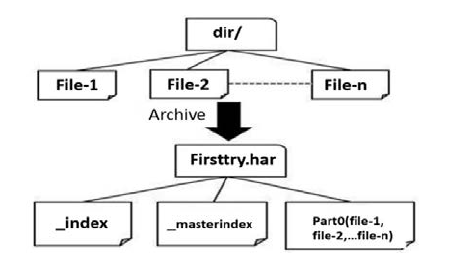
\includegraphics{DataModelforArchivingSmallFiles.PNG}
\caption{Data Model for Archiving Small Files}
\label{fig:DataModelforArchivingSmallFiles}
\end{figure}

创建一个HAR将会减少在NameNode的数据量,并且也会减少在mapreduce里面的map操作,提高性能。如图 \ref{fig:DataModelforArchivingSmallFiles}

创建一个HAR文件:可以通过使用Hadoop 归档命令:

hadoop archive -archiveName name -p [parent] [src] [dest]

这个命令会运行一个map reduce把文件打包成少量的HDFS文件。读取在HAR中的文件会比直接读HDFS文件要低效,但是升级HAR需要改变HDFS结构,这个会很困难。


\subsubsection{Improved HDFS}
改进的HDFS结构\cite{ChenJ}包括两个部分:

\begin{itemize}
\item 客户端部分,整合小文件到一个大文件。
\item 数据节点部分,满足缓存源管理
\end{itemize}

\begin{figure}[h]
\centering
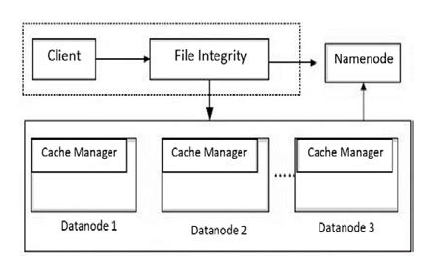
\includegraphics{ImprovedHDFSFramework.PNG}
\caption{Improved HDFS Framework}
\label{fig:ImprovedHDFSFramework}
\end{figure}

图 \ref{fig:ImprovedHDFSFramework}表现了这两点。改进的HDFS模型是基于索引的,属于同一个目录的文件会被整合到一个大文件,然后为每一个小文件建立索引,相应地减少了NameNode的负担。缓存机制则提高了小文件的读取效率,缓存管理是在DataNode里面的,当读取一个小文件的时候,在缓存里面的数据首先会被搜索。

每一个整合的大文件都有一个索引文件,包含了偏移量和每个原小文件的长度。整合的步骤如下:

\begin{itemize}
\item 在每个目录里,根据文件的大小排序,然后把一个接一个把小文件写入大文件里面
\item 确定所有小文件的总和
\item 确定大文件的大小,然后把结果和HDFS块的大小进行比较
\end{itemize}

索引文件是依据偏移量和每个小文件的大小来创建的,为了把这个大文件存储在一个块里,文件大小应该小于块的大小。如果比它大,就会分割成几个块。


\subsubsection{Extended HDFS}
这个方法\cite{Gurav}扩展了HDFS并且被命名为 Extended HDFS(EHDFS). EHDFS是基于索引的,当小文件的数目过于庞大,就会使索引文件很大,更新它会很困难。为了提高读取效率,使用了预取机制。EHDFS 提供了一个改进的索引机制,以及预取索引信息。它有四个技术起了决定性作用:文件合并(file merging)、文件映射(file mapping)、预取(prefetching)、抽取(extraction). 图\ref{fig:ExtendedHDFSArchitecture}表现了这几点。

\begin{figure}[h]
\centering
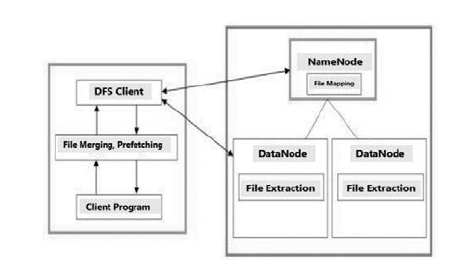
\includegraphics{ExtendedHDFSArchitecture.PNG}
\caption{Extended HDFS Architecture}
\label{fig:ExtendedHDFSArchitecture}
\end{figure}

\emph{File Merging}
在文件合并的时候,NameNode只会保存大文件而不是里面所有的小文件,除了文件数据,一个索引表也会被放在每个块的开头,这张表包含了每个小文件的条目,每个表条目都是一个pair(offset, length),文件合并后的块的结构如图\ref{fig:BlockStructureAfterFileMerging},
DataNode里面块的储存如图\ref{fig:StructureofAnExtendedBlock}

\begin{figure}[h]
\centering
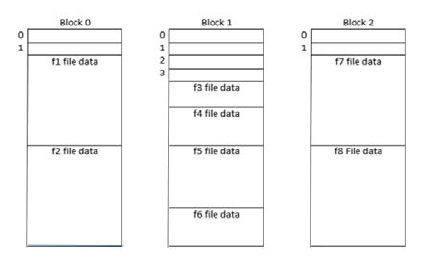
\includegraphics{BlockStructureAfterFileMerging.PNG}
\caption{Block Structure After File Merging}
\label{fig:BlockStructureAfterFileMerging}
\end{figure}


\begin{figure}[h]
\centering
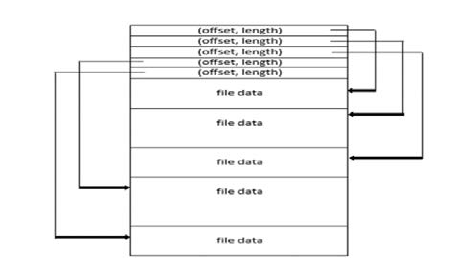
\includegraphics{StructureofAnExtendedBlock.PNG}
\caption{Structure of an Extended Block}
\label{fig:StructureofAnExtendedBlock}
\end{figure}

\emph{File Mapping}
文件映射是由NameNode完成的,文件映射意思是,将小文件的名字映射到包含这个小文件的合并文件上,为了获取所需的小文件的位置,一个包含小文件和合并文件名字的请求被发送到NameNode. 对每个合成文件,NameNode都包含了一个称为Constituent File Map的数据结构,小文件名字和包含这个小文件的合成文件的逻辑块号被映射。NameNode也提供了一个索引条目号在块的开头。


\emph{Prefetch}
文件合并不会提高读取的性能,它只会减少元数据的量,使用预取可以优化这一点,无论何时客户端试图读取一个小文件的时候,在同一个块的其他小文件的元数据都会被预取下来。

\emph{File Extraction}
由DateNode执行,将制定文件从一个块中提取出来。当读取一个文件的时候,客户端需要明确小文件的名字和合成文件的名字,用这两个信息去获取:包含这个文件的块、包含这个块的DataNode、在NameNode里面的索引表。


\subsubsection{New HAR}
关于NHAR\cite{Nupairoj}的基本想法包括如下两点:

\begin{itemize}
\item 合并小文件到大文件,去减少文件的数目,优化存取性能
\item 扩展HAR的文件管理功能,让它更像典型的文件系统
\end{itemize}

NHAR重构了索引结构去改善HDFS的元数据主框架以及文件存取性能,新的设计使得NHAR可以新加的文件被添加到现存的归档上。当从HAR读取文件的时候,需要两次获取索引,为了改善这一点,NHAR使用单层索引,NHAR使用索引信息去创建一个哈希表而不是使用主索引方式。将一个新文件添加到HAR文件里面,需要创建一个新HAR文件,但是NHAR不需要重构一个新文件,它只需要归档新文件,合并索引文件,移动新部分文件。

\subsubsection{小结}
这几种方法在\cite{Sachin}中已经总结,基本上是2012-2014年发表的,从2017年发表的相关论文来看,近期的很多论文都是在早期一些实践基础上的改进,包括算法的改良,以及适用于不同领域的方法。

\subsection{想法及可能遇到的挑战}
综合所看的大量文献来看,可能下一步从以下几个方向寻找突破口:

\begin{itemize}
\item 依据文件的属性特征、系统特征、用户需求决定使用何种策略。这一点启发来自2017年这篇文章\cite{Lidong}使用决策树对几种分布式文件系统(Ceph, HDFS, GlusterFS)进行选择, 以此实现依照不同文件属性来选择何种DFS. 
\item 考虑用户的读取特征,由概率特征或者行为模式建立机器学习算法优化EHDFS策略。这个启发来自\cite{TaoW},以前的优化策略仅仅考虑DFS结构本身,而忽略了用户的行为,这篇文章中,使用了概率预测,来优化合并和预取机制,其他部分基本类似上文的EHDFS.
\item 特定文件存取的优化。没有一个策略是完全适用所有情况的,在这篇\cite{DongB}文章中,作者只对PPT的存取进行优化,由此观之,也可以对其他特定的、常用的、急于解决的文件存取进行优化。
\end{itemize}

\subsection{新思路}
\subsubsection{对上文的总结}
上文针对DFS做了详细的介绍,并且指出了DFS的存取问题,特别地,选择了一个通用性比较强的HDFS作为主要研究对象,探讨了它相关的问题,以及自从问题出现以来,各种的解决思路。在各路优化策略之后,是否仍有进步的空间?以及这样解决问题的方法是否仅仅适用于HDFS?

在\cite{Milad}的启发下,我们做了如下的分析

\subsubsection{基于预测的文件预取}
在上文指出,大部分分布式文件系统有这样的特点,即:写一次读多次,那么去解决读取的问题会有更大的价值以及进步空间。要解决读取的问题,就是要解决读取速度的问题,类似于使用多级缓存,在DFS中要解决的问题就是如何准确地把文件预取到本地文件系统,最终关于预取的问题,就是关于预测的问题。

结合上文,我们把问题缩小到对小文件的读取预测。当用户需要读取大量小文件的时候,特别是长时间对文件进行读取的时候,可以通过学习读取模式来预测下一步可能的内容,再通过预取,等到用户用到该文件的时候可以更加节省时间。

\subsubsection{类比内存读取}
给定一个设计,为了最大化效率,计算机结构总是会使用预测,预取是一个典型的案例,这个指的是,指令或者数据在它们被使用之前加载到更快的储存里面,在DFS方面,远程的存储相当于较慢的一面,而本地储存相当于较快的一面。在内存方面,冯诺伊曼体系有一个非常重要的瓶颈,即计算是存取数据的指数级倍数,这个问题被称为memory wall. 有文章指出,现代应用会耗费一般的时钟周期等待数据从内存取出来,同样的问题也摆在了DFS方面。为了克服这个问题,处理器使用了层次化的内存系统结构,使更小的更快速的存储更加靠近处理器,使大容量的慢速的较远。这种结构完全类似DFS. 在这种情况下,预取器会预测何时取数据到cache,那么核心问题就是预测内存读取模式。

现代的处理器使用了很多种预测结构,从历史来看,几乎全部的预取器是基于表结构的。也就是说,未来的事件和之前的访问历史相关。但是,当working set比predictive table大得多的时候,效率会显著下降。类比到DFS,使用DFS的目的就是存储大量的数据文件,也就是working set非常大,而使用它的时候,只会使用其中的一部分数据。所以使用其他方法来预测就显得很有必要了。

\subsubsection{使用神经网络}
当前神经网络作为一个强大的技术在序列预测问题方面,比如说自然语言处理,文本理解。而在DFS预测预取方面使用神经网络目前没有看到任何相关的研究,因而本次研究是首次的。

对此做几点说明
\begin{enumerate}
\item 普通的深度神经网络主要针对标准化的数据,比如固定长度的特征向量或者图片转化成的RGB张量,对于序列化的数据使用RNN已经有了很多的应用。针对RNN的梯度消失和梯度爆炸问题,学界给出的改进LSTM则解决了这个问题。
\item 普通的预测问题可以看成回归问题,但是对于海量小文件的问题,由于数量非常大,而且目标很稀疏,此时传统的回归学习已经非常不适用了。
\item 使用神经网络必然会增加时间的开销,这也是我们所担心的一个问题,但是考虑到目前已经有相关的神经网络加速手段,比如FPGA,而我们仅仅只用做一个开端性的工作即可。
\item 目前神经网络发展迅速,已经不需要自己从零开始构建,我们打算使用现有的库keras(tensorflow作为底层)来搭建。
\item 考虑到时间的因素,我们以准确率作为主要的度量。
\end{enumerate}

除此之外,可能会遇到以下的几点问题
\begin{itemize}
\item 神经网络准确率优化困难
\item 数据集的寻找或者构建
\item DFS和神经网络的结合
\end{itemize}



\begin{thebibliography}{99}
\bibitem{Dhruba} Dhruba Borthakur :\emph{The Hadoop Distributed File System: Architecture and Design}  Hadoop Project Website.
\bibitem{Songling}Songling Fu, Ligang He:\emph{Performance Optimization for Managing Massive Numbers of Small Files in Distributed File Systems} IEEE TRANSACTIONS ON PARALLEL AND DISTRIBUTED SYSTEMS, VOL. 26, NO. 12, DECEMBER 2015 3433
\bibitem{Sachin}Sachin Bendea, Rajashree Shedge:\emph{Dealing with Small Files Problem in Hadoop Distributed File System} Procedia Computer Science 79 ( 2016 ) 1001 – 1012
\bibitem{Xiaojun}XiaoJun Liu, Chong Peng, ZhiChao Yu:\emph{Research on the Small Files Problem of Hadoop} International Conference on Education, Management, Commerce and Society (EMCS 2015)
\bibitem{Korat}Korat, V.G., Pamu, K.S., \emph{Reduction of Data at Namenode in HDFS using HAR Technique}, International Journal of Advanced Research in Computer Engineering and Technology, Vol.1, pp.635-642, June 2012.
\bibitem{ChenJ}Chen, J., Wang, D., Fu, L., and Zhao, W., \emph{An Improved Small File Processing Method for HDFS}, International Journal of Digital Content
Technology and its Applications (JDCTA), Vol.6, pp.296-304, Nov 2012
\bibitem{Gurav}Gurav, Y.B., Jayakar, K.P., \emph{Efficient Way for Handling Small Files using Extended HDFS}, International Journal of Computer Science and
Mobile Computing, Vol.3, pp.785-789, June 2014
\bibitem{Nupairoj}Nupairoj, N., Vorapongkitipun, Chatuporn., \emph{Improving Performance of Small-File Accessing in Hadoop}, 11th International Joint
Conference on Computer Science and Software Engineering, pp.200-205, May 2014.
\bibitem{Lidong}Lidong Zhang, Yongwei Wu, Ruini Xue, Tse-Chuan Hsu, Hongji Yang, Yeh-Ching Chung:\emph{HybridFS - A High Performance and Balanced File System Framework with Multiple Distributed File Systems}2017 IEEE 41st Annual Computer Software and Applications Conference
\bibitem{TaoW}Tao Wang, Shihong Yao, Zhengquan Xu, Lian Xiong, Xin Gu, Xiping Yang \emph{An Effective Strategy for Improving small file problem in Distributed file system}, International Conference on Information Science and Control Engineering, pp.122-126, 2015
\bibitem{DongB}Dong, B., Qiu, J., Zheng, O., Zhong, X., Li, J., Li, Y.: \emph{A novel approach to improving the efficiency of storing and accessing small files on Hadoop: a case study by powerpoint files} In: Proceedings of International Conference on Services Computing, pp. 65–72 (2010) 
\bibitem{Milad}Milad Hashem Kevin Swersky: \emph{Learning Memory Access Patterns} arXiv:1803.02329v1 [cs.LG] 6 Mar 2018
\end{thebibliography}

\end{document}